\section*{Resultados da execução final otimizada}

O protocolo final usa exclusivamente trajetórias de 1.000 eventos, com
75.000 amostras de treino, 10.000 de validação e 15.000 de teste.
As redes são resumidas sobre cinco seeds independentes; o MLE é ajustado
separadamente em cada trajetória do mesmo conjunto de teste.
Os intervalos das redes usam a distribuição $t$ de Student entre seeds.

\begin{table}[htbp]
\centering
\caption{Métricas agregadas no teste sintético congelado (15.000 trajetórias de 1.000 eventos).}
\label{tab:final-agregado}
\small
\begin{tabular}{lrrrrr}
\toprule
Estimador & MSE macro & IC 95\% & MAE macro & MSE de $g$ & Validade\\
\midrule
LSTM & 0,019618 & [0,013252; 0,025984] & 0,094276 & 0,001825 & 100,00\%\\
Transformer & 0,023700 & [0,019128; 0,028272] & 0,105642 & 0,002138 & 100,00\%\\
MLE & 0,506193 & -- & 0,111852 & 0,002344 & 100,00\%\\
\bottomrule
\end{tabular}
\end{table}

\begin{table}[htbp]
\centering
\caption{MSE de teste por parâmetro (redes: média de cinco seeds).}
\label{tab:final-parametros}
\begin{tabular}{lrrrr}
\toprule
Estimador & $\mu$ & $\alpha_{\mathrm{self}}$ & $\alpha_{\mathrm{cross}}$ & $\beta$\\
\midrule
LSTM & 0,002296 & 0,016222 & 0,016566 & 0,043386\\
Transformer & 0,002366 & 0,020905 & 0,021196 & 0,050332\\
MLE & 0,010108 & 0,006146 & 0,006214 & 2,002303\\
\bottomrule
\end{tabular}
\end{table}

\begin{table}[htbp]
\centering
\caption{MSE macro por regime da razão de ramificação $g$.}
\label{tab:final-regimes}
\begin{tabular}{lrrr}
\toprule
Estimador & $g$ baixo & $g$ intermediário & $g$ quase crítico\\
\midrule
LSTM & 0,019941 & 0,015614 & 0,023297\\
Transformer & 0,022228 & 0,018964 & 0,029908\\
MLE & 1,480568 & 0,016795 & 0,021214\\
\bottomrule
\end{tabular}
\end{table}

Entre as redes, a LSTM obteve MSE macro médio 17,2\% menor que o Transformer.
Com 5 e 5 seeds, porém, a diferença não é estatisticamente significativa (teste de Welch, $p=0,19$), e os intervalos de confiança se sobrepõem; os dados não permitem ordenar as redes.
No MLE, o parâmetro $\beta$ respondeu por 98,9\% da soma dos erros quadráticos,
e o MSE macro no regime de $g$ baixo foi 88,15 vezes o do regime intermediário:
com excitação fraca, $\beta$ é pouco identificado e algumas trajetórias
produzem estimativas extremas. Fora desse regime, o MLE é competitivo:
no regime intermediário, seu MSE macro foi 0,0168 (LSTM: 0,0156; Transformer: 0,0190) e, no
quase crítico, 0,0212 (LSTM: 0,0233; Transformer: 0,0299).
O MLE obteve o menor MSE entre os três estimadores em $\alpha_{\mathrm{self}}$ e $\alpha_{\mathrm{cross}}$.
Portanto, o MSE macro agregado não ordena os estimadores de forma robusta,
e convergência numérica não implica boa recuperação paramétrica.

\begin{figure}[htbp]
\centering
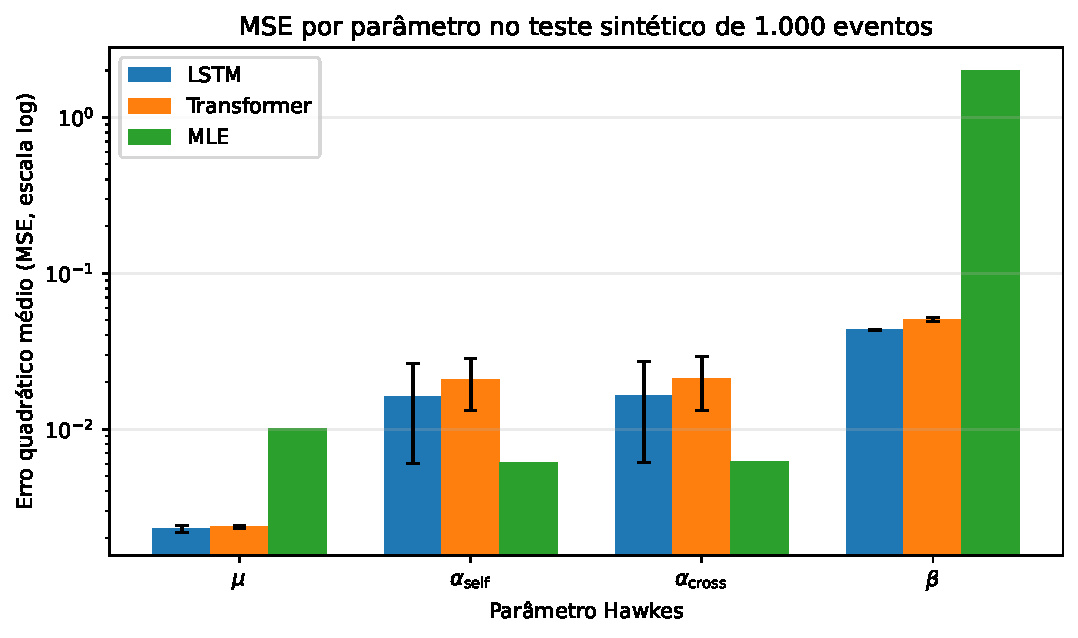
\includegraphics[width=0.88\linewidth]{../build/figures/parameter_mse.pdf}
\caption{MSE de teste por parâmetro no protocolo de 1.000 eventos.
As barras de erro das redes representam um desvio-padrão entre seeds.}
\end{figure}

\begin{figure}[htbp]
\centering
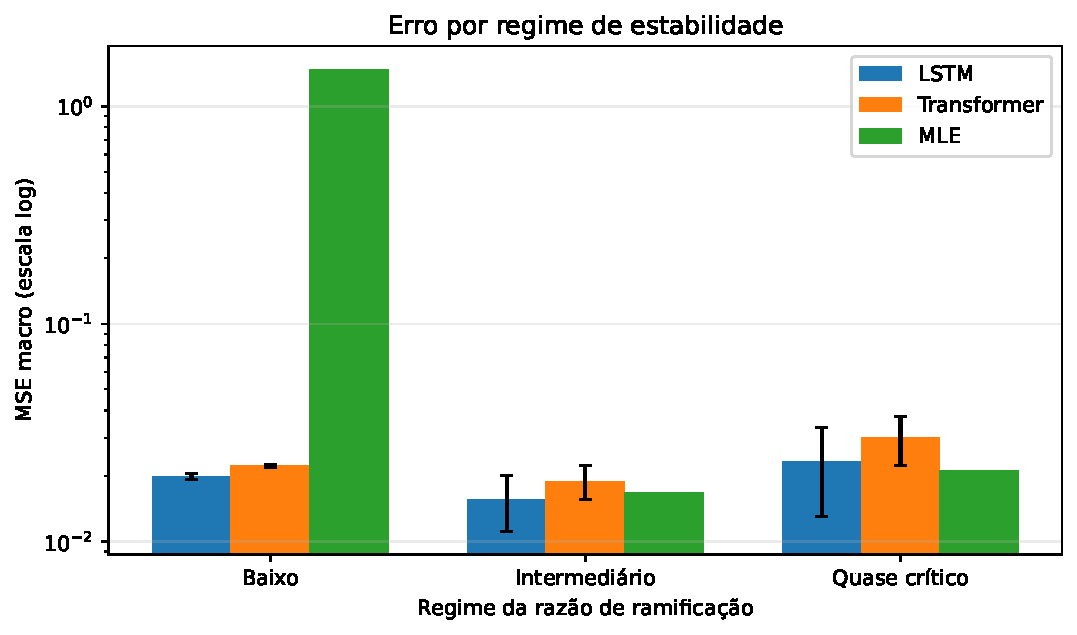
\includegraphics[width=0.88\linewidth]{../build/figures/branching_regime_mse.pdf}
\caption{MSE macro por regime da razão de ramificação. As barras de erro
das redes representam um desvio-padrão entre seeds.}
\end{figure}

\begin{figure}[htbp]
\centering
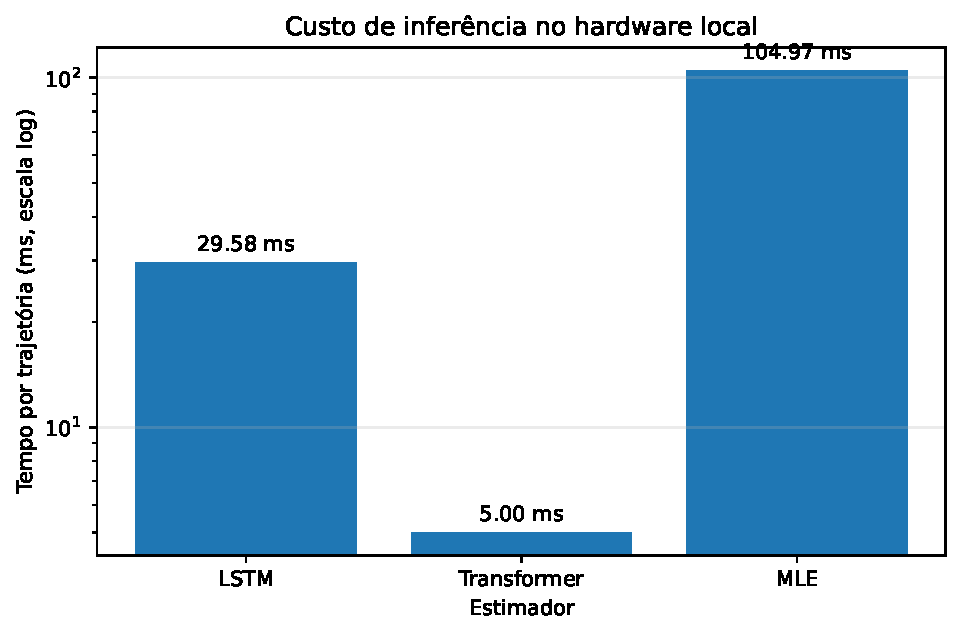
\includegraphics[width=0.80\linewidth]{../build/figures/inference_cost.pdf}
\caption{Custo por trajetória registrado durante a execução final, em escala
logarítmica. Para o MLE, tempo de parede com quatro processos que concorriam
com o treino na GPU; para as redes, latência mediana em batch unitário no
MPS. Um benchmark controlado posterior mediu cerca de 10~ms por trajetória
para o MLE em um único núcleo e deve ser preferido a esta figura.}
\end{figure}

O MLE convergiu em 100,00\% das trajetórias
e usou mediana de 14,00 iterações.
Todas as comparações usam o mesmo conjunto de teste congelado.
